\chapter{Materiais e Métodos}

\section{Procedimentos Experimentais}
A partir da classe com menor representatividade na base de dados, classe 4 - Algodão Americano/Salgueiro com 2.747 observações, sendo todos os dados selecionados, foram extraídas das outras seis classes de tipos de cobertura florestal 2.747 observações, selecionadas aleatoriamente com o auxilio do software R, totalizando o conjunto de teste com 19.229 observações, conforme a tabela \ref{tb:dados}.

\begin{table}[htbp]
\caption{Observações Selecionadas}
\label{tb:dados}
\centering
\setlength{\tabcolsep}{5pt}
\begin{tabular}{cccccc}
\hline
Tipo de Cobertura  &Total de  &Observações  &Porcentagem por \\
Florestal &Observações &Selecionadas &Tipo de Cobertura \\
\hline
Classe 1 &211.840 &2747 &1,29\% \\
Classe 2 &283.301 &2747 &0,97\% \\
Classe 3 &35.754  &2747 &7,68\% \\
Classe 4 &2.747   &2747 &100\% \\
Classe 5 &9.493   &2747 &28,94\% \\
Classe 6 &17.367  &2747 &15,82\% \\
Classe 7 &20.510  &2747 &13,39\% \\
\hline
\textbf{Total} &\textbf{581.012} &\textbf{19.229} &\textbf{3,31\%} \\
\hline
\end{tabular}
\\
\singlespacing
\text{\footnotesize Fonte: O autor}
\end{table}


\begin{figure}[htb]
\centering
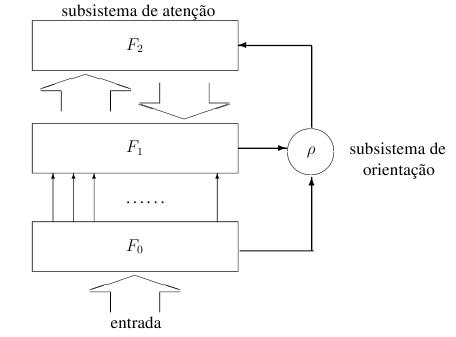
\includegraphics[scale=.5]{art}
\caption{Arquitetura da rede neural ART}\label{fig:art}
\end{figure}
\section{Análise dos Dados}


\section{Cronograma}
Visando atingir os objetivos propostos apresenta-se um cronograma
de atividades a ser realizado no âmbito do Departamento de
Automação e Sistemas (DAS/UFSC). Estas atividades e o cronograma
estão ilustrados nas tabelas \ref{tb:atividades} e
\ref{fig:cronograma}, respectivamente.

%%%% INICIO ATIVIDADES PREVISTAS %%%%%%%%%%%%%%%%%

\begin{table}[!htb]
  \centering
  \caption{Atividades Previstas}\label{tb:atividades}
  \begin{tabular}{cp{12cm}}
    \hline \hline &\\[-0.4cm]
    {\bf Atividades} & \multicolumn{1}{c}{\bf Descrição} \\
    \hline
    &\\[-0.4cm]
    \textbf{A} & Revisão bibliográfica. \\[0.2cm]
    \textbf{B} &  Estudo de novas representações.\\[0.2cm]
    \textbf{C} &  Aplicação dos algoritmos.\\[0.2cm]
    \textbf{D} &  Desenvolvimento da interface. \\[0.2cm]
    \textbf{E} &  Validação dos resultados.\\[0.2cm]
    \textbf{F} &  Elaboração da monográfia.\\[0.2cm]
    \textbf{G} &  Defesa.\\[0.2cm]
    \hline \hline
  \end{tabular}
\end{table}

%\begin{preview}
%\centering

\begin{figure}

  \begin{gantt}{10}{12}
    \begin{ganttitle}
    \numtitle{1}{1}{12}{1}
    \end{ganttitle}
    \ganttbar{Revisão da literatura}{0}{2}
    \ganttbarcon{refinamento método}{2}{5}
    \ganttbarcon{}{8}{2}
    \ganttmilestone[color=cyan]{Milestone with color!}{4}
    \ganttbar{another task}{2}{2}
    \ganttbar[color=cyan]{another coloured task}{4}{4}
    \ganttbar{another task}{4}{2}
    \ganttcon{4}{5}{4}{7}
    \ganttmilestonecon{A connected Milestone}{7}
    \ganttbarcon{another consecutive task}{8}{2}
  \end{gantt}
%\end{preview}
\caption{Cronograma de Atividades}\label{fig:cronograma}
\end{figure}
\section{Recursos}
Descrever os recursos necessários para o desenvolvimento da pesquisa.
\subsection{Recursos Humanos}
\subsection{Recursos Físicos}


